\documentclass{math201}
\usepackage{hyperref}
\usepackage{bookmark}
\usepackage{minted}

% =============================================
% Part 0 信息
% =============================================

\mathsetup{
  % 学生姓名
  student = {某同学},
  % 学号
  student-id = {2021xxxx},
  % 院系
  experiment = {实验二 外部中断实验},
  % 专业年级
  discipline = {集成电路设计与集成系统},
  % 日期
  date = {\today},
}

\begin{document}

% =============================================
% Part 1  封面
% =============================================

\makecover

% =============================================
% Part 2 主文档
% =============================================

\section{实验要求}

\begin{enumerate}
  \item 运行例程\textbf{实验4 EXTI外部中断实验},分別按下key1/key2键,观察实验现象
  \item 看懂源程序
  \item 修改源程序、实现按下key1键,红灯、黄灯,绿灯披顺序亮,按下key2键,绿灯。黄灯,红灯按顺序亮。红灯亮时蜂鸣器响。
  \item 完成实验报告,把修改的程序截图、实验现象截图或者图片整理到报告中。
\end{enumerate}

\section{实验内容及结果}

\subsection{编写代码}

需要修改 \textbf{stm32f4xx\_it.c} 中的 \textbf{void KEY1\_IRQHandler(void)}

首先修改\textbf{main.c},初始化蜂鸣器等

\inputminted[
    frame=lines,
    framesep=2mm,
    baselinestretch=1.2,
    fontsize=\small,
    linenos
]{C++}{code/main.c}

然后修改\textbf{stm32f4xx\_it.c},添加中断处理函数

\inputminted[
    frame=lines,
    framesep=2mm,
    baselinestretch=1.2,
    fontsize=\small,
    linenos
]{C++}{code/stm32f4xx_it.c}

\subsection{下载运行}

使用 \texttt{FlyMCU.exe} 下载程序到 STM32 开发版上,观察实验现象。

\subsection{实验现象}

\begin{figure}[H]
  \centering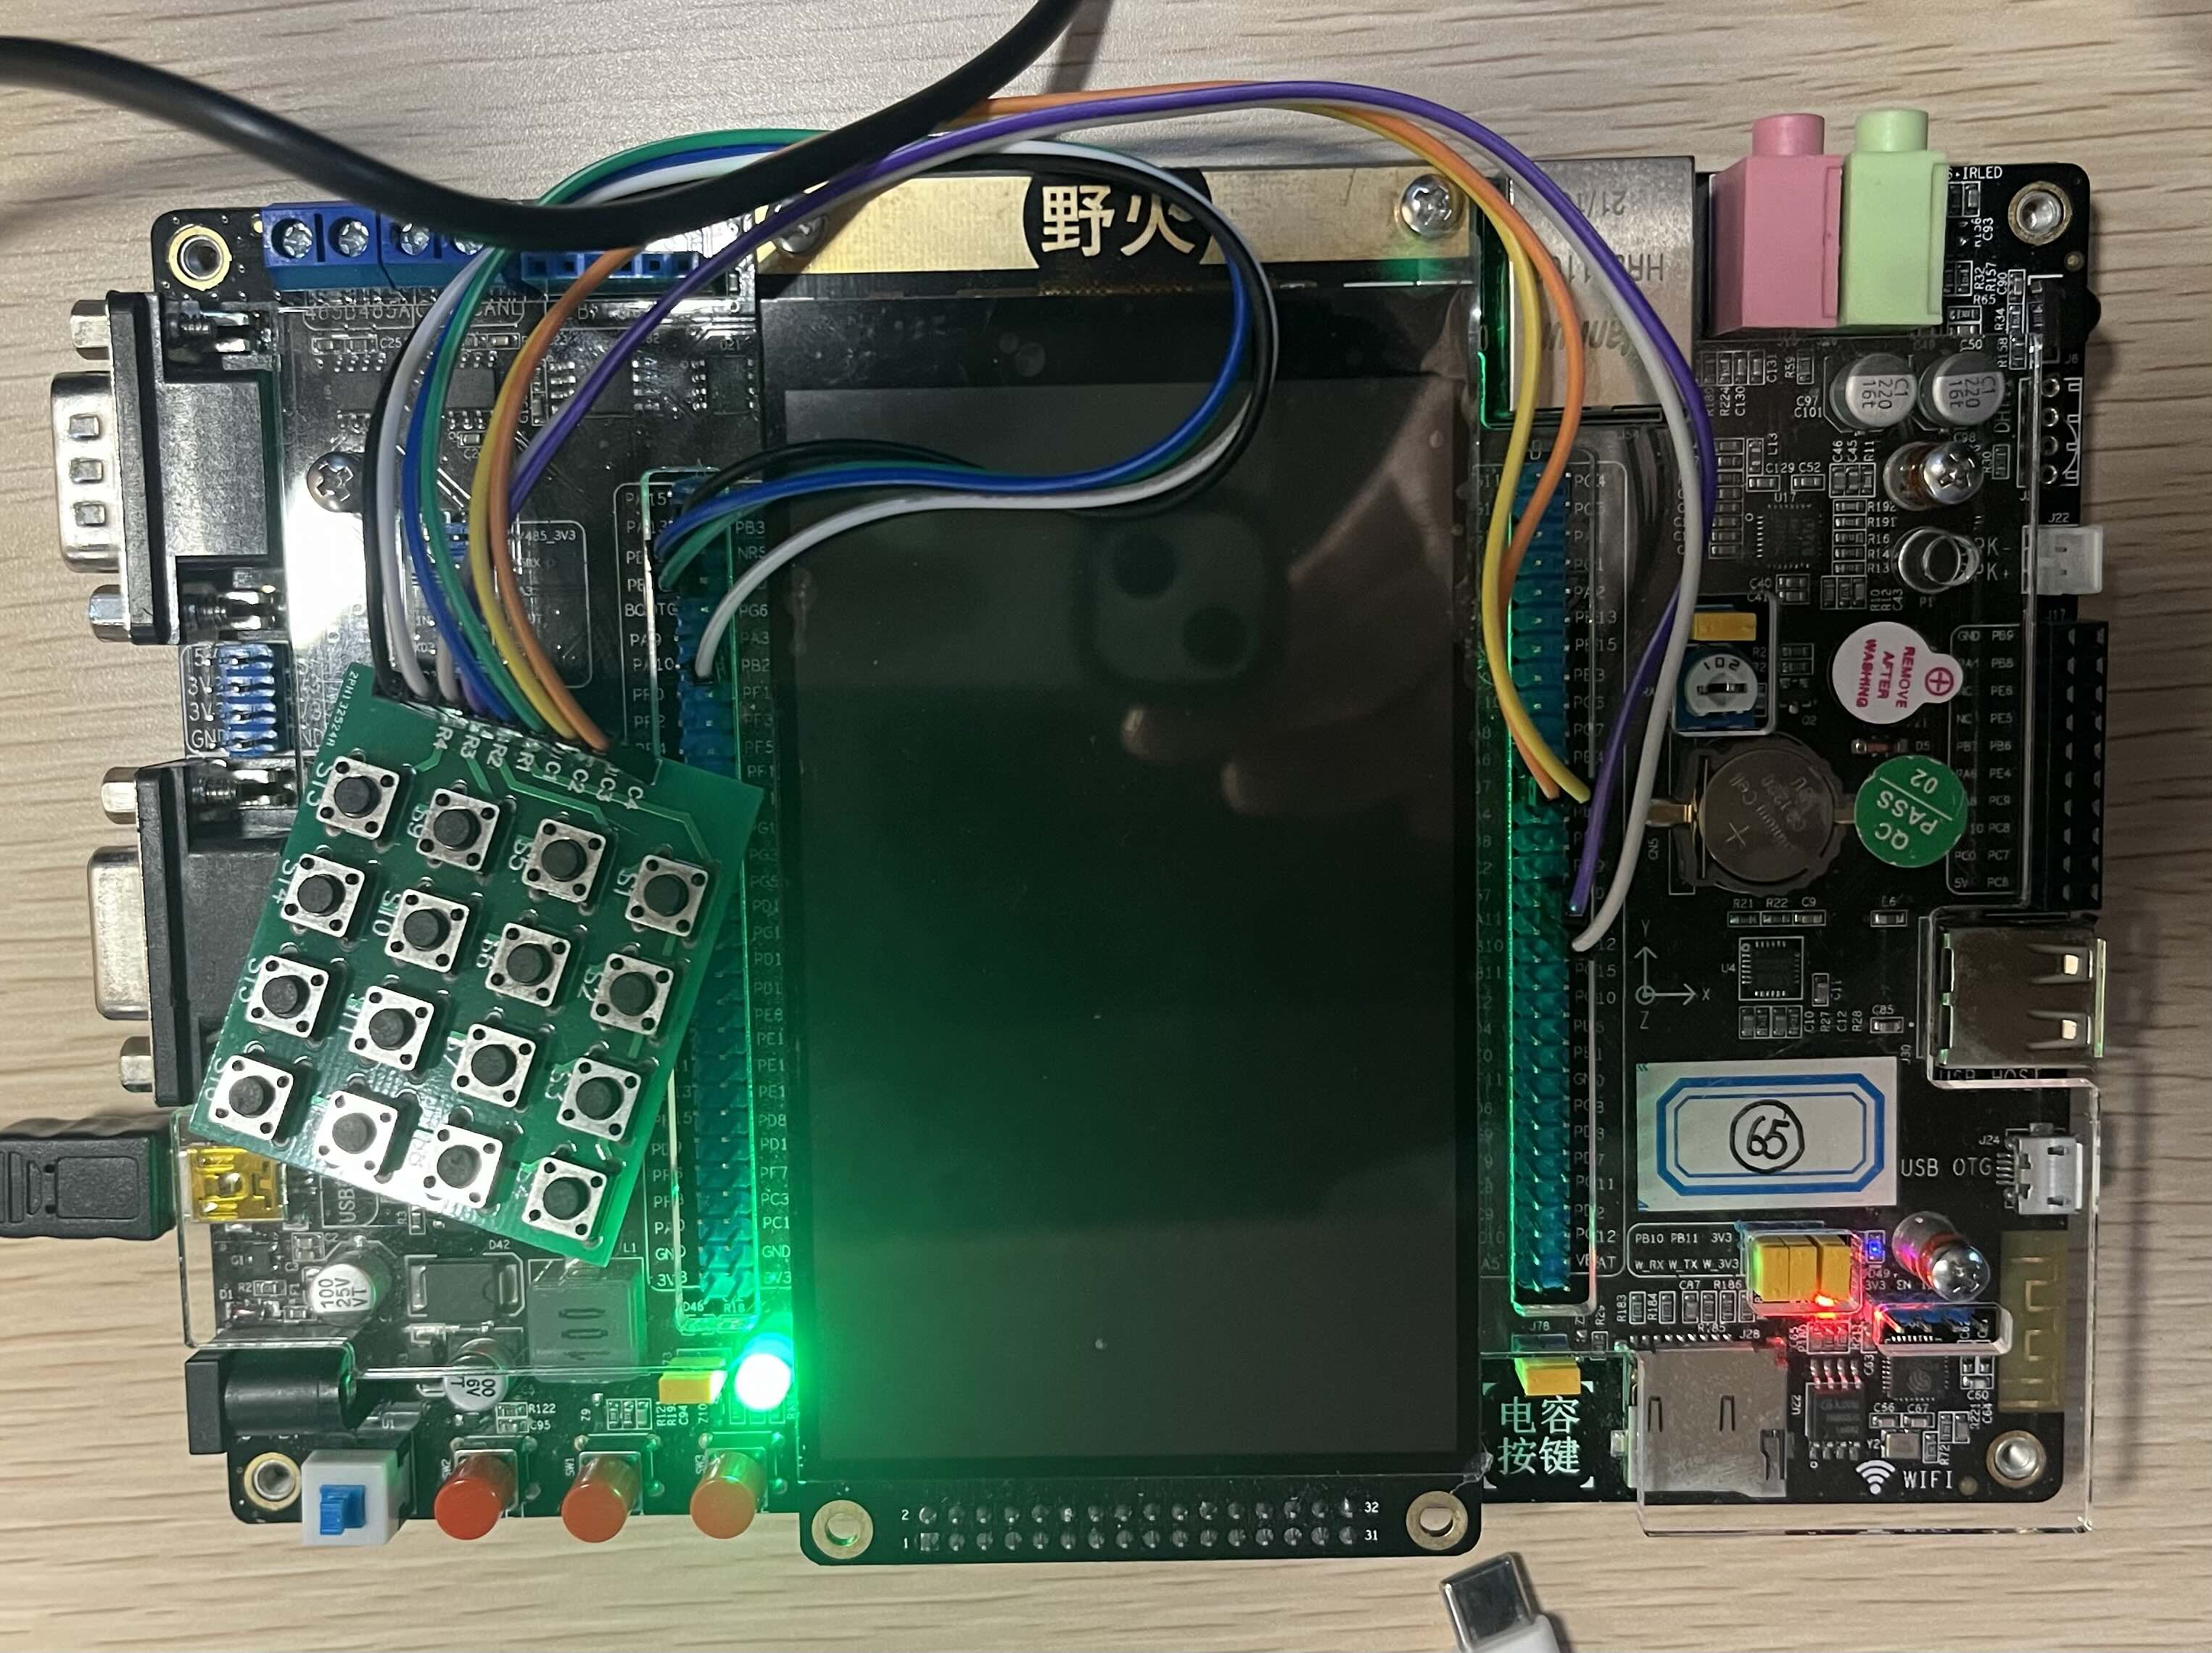
\includegraphics[width=0.6\linewidth]{led_green.jpg}
  \caption{绿灯亮}      
\end{figure}

\begin{figure}[H]
  \centering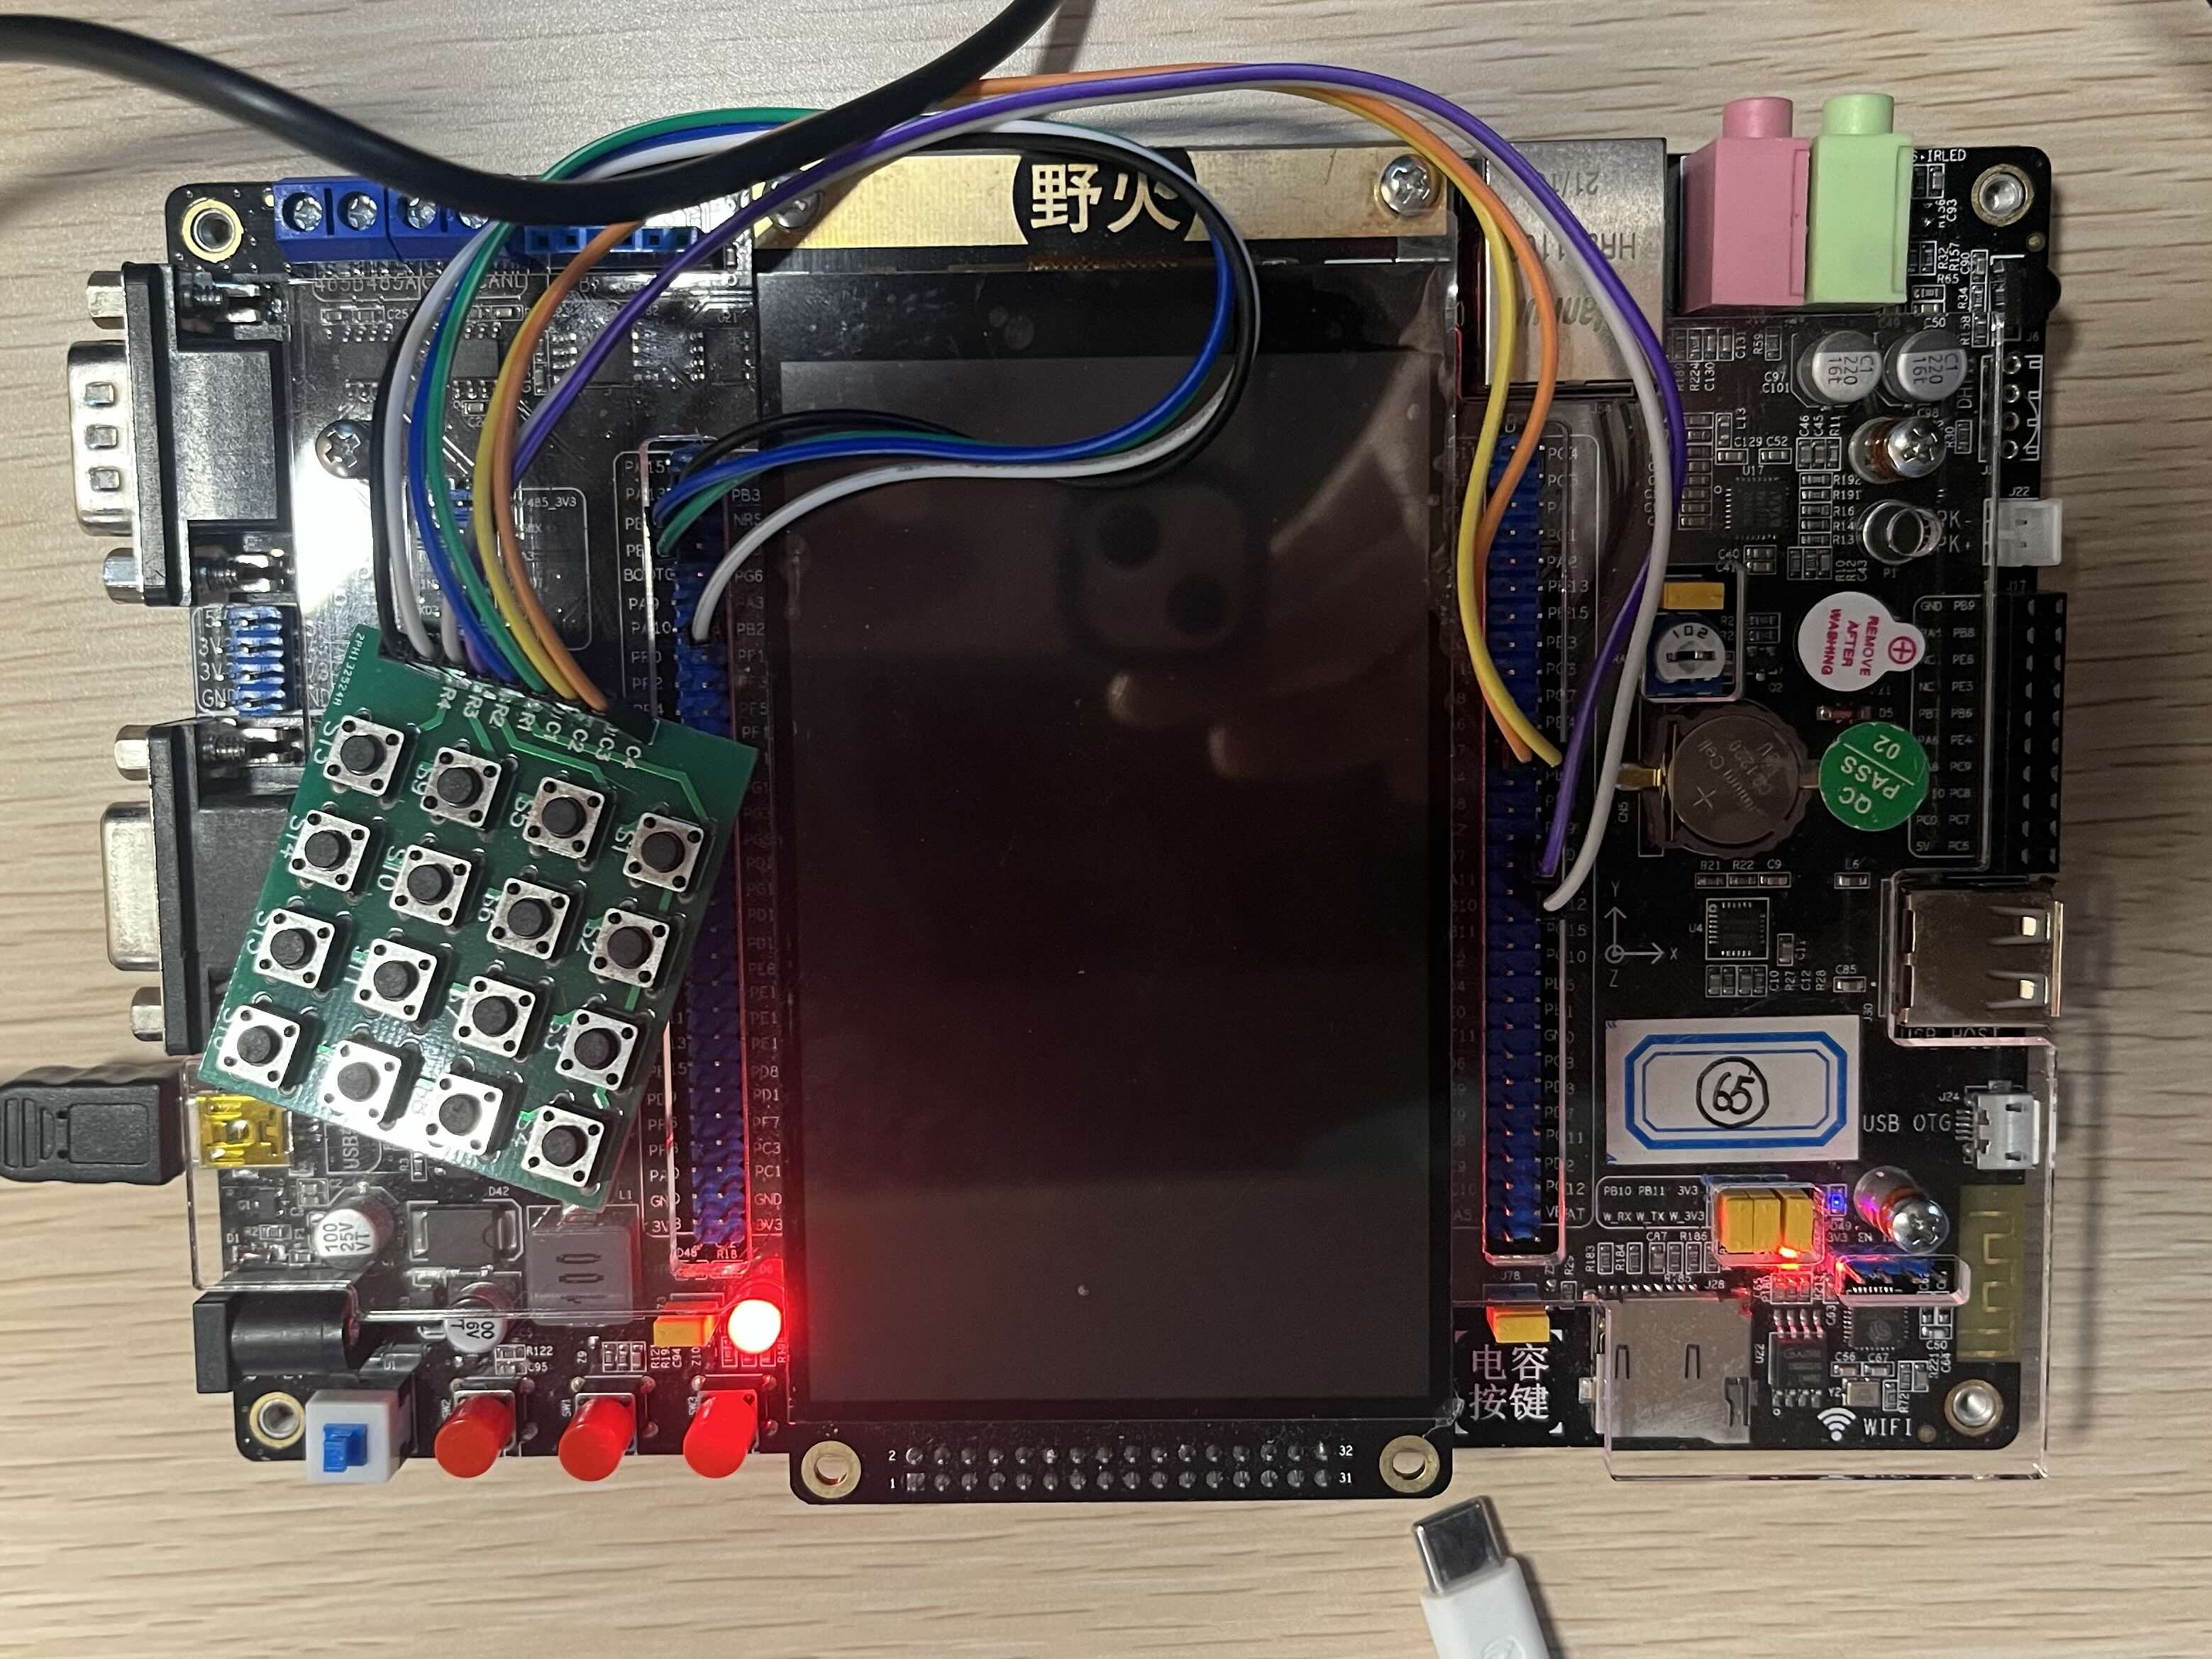
\includegraphics[width=0.6\linewidth]{led_red.jpg}
  \caption{红灯亮}
\end{figure}

\section{实验小结}

\begin{enumerate}
  \item 按下key1键,红灯、黄灯、绿灯依次亮起。
  \item 按下key2键,绿灯、黄灯、红灯依次亮起,且红灯亮时蜂鸣器响。
\end{enumerate}

通过本实验,掌握了STM32外部中断的配置和使用,并能够根据实际需求修改程序实现相应功能。

\end{document}
